% Copyright 2004 by Till Tantau <tantau@users.sourceforge.net>.
%
% In principle, this file can be redistributed and/or modified under
% the terms of the GNU Public License, version 2.
%
% However, this file is supposed to be a template to be modified
% for your own needs. For this reason, if you use this file as a
% template and not specifically distribute it as part of a another
% package/program, I grant the extra permission to freely copy and
% modify this file as you see fit and even to delete this copyright
% notice. 

% \UseRawInputEncoding
\documentclass{beamer}

% There are many different themes available for Beamer. A comprehensive
% list with examples is given here:
% http://deic.uab.es/~iblanes/beamer_gallery/index_by_theme.html
% You can uncomment the themes below if you would like to use a different
% one:
%\usetheme{AnnArbor}
%\usetheme{Antibes}
%\usetheme{Bergen}
%\usetheme{Berkeley}
%\usetheme{Berlin}
%\usetheme{Boadilla}
%\usetheme{boxes}
%\usetheme{CambridgeUS}
%\usetheme{Copenhagen}
%\usetheme{Darmstadt}
%\usetheme{default}
%\usetheme{Frankfurt}
%\usetheme{Goettingen}
%\usetheme{Hannover}
%\usetheme{Ilmenau}
%\usetheme{JuanLesPins}
%\usetheme{Luebeck}
\usetheme{Madrid}
%\usetheme{Malmoe}
%\usetheme{Marburg}
%\usetheme{Montpellier}
%\usetheme{PaloAlto}
%\usetheme{Pittsburgh}
%\usetheme{Rochester}
%\usetheme{Singapore}
%\usetheme{Szeged}
%\usetheme{Warsaw}

\usepackage{pgfgantt}
\usepackage{todonotes}
\usepackage{media9}
\usepackage{subfigure}
\usepackage{booktabs,array}
\usepackage[font=tiny,labelfont=bf]{caption}
\usepackage{tabulary}
\usepackage{caption}
\usepackage{graphicx}
\usepackage{siunitx}
\usepackage{arydshln}


% Customize Warsaw color 
\setbeamercolor*{palette primary}{use=structure,fg=white,bg=red!50!black}
\setbeamercolor*{palette secondary}{use=structure,fg=white,bg=red!60!black}
\setbeamercolor*{palette tertiary}{use=structure,fg=white,bg=red!70!black}

% Customize Warsaw block title and background colors
\setbeamercolor{block title}{bg=red!50!black,fg=white}

\setbeamertemplate{navigation symbols}{} % Remove navigation symbols
\setbeamertemplate{bibliography item}{\insertbiblabel}  % insert bibliography numbers instead of symbol
\setbeamertemplate{caption}[numbered] % adds the figure or table number to the caption.

% Set up footer manually
\setbeamertemplate{footline}
{
  \leavevmode%
  \hbox{%
  \begin{beamercolorbox}[wd=.45\paperwidth,ht=2.25ex,dp=1ex,center]{author in head/foot}%
    \usebeamerfont{author in head/foot}\insertshortauthor\hspace*{1em}(\insertshortinstitute)
  \end{beamercolorbox}%
  \begin{beamercolorbox}[wd=.4\paperwidth,ht=2.25ex,dp=1ex,center]{title in head/foot}%
    \usebeamerfont{title in head/foot}\insertshorttitle
  \end{beamercolorbox}%
  \begin{beamercolorbox}[wd=.15\paperwidth,ht=2.25ex,dp=1ex,center]{date in head/foot}%
    \usebeamerfont{date in head/foot}\insertframenumber{} / \inserttotalframenumber
  \end{beamercolorbox}}%
  \vskip0pt%
}

%==============================================================================
%     TITLE
%==============================================================================
\title[Smart Robotic Cart]{Smart Robotic Cart: A Prototype}

\author[K.~Allen, D.~Beebe, J.~Braker]{Kallistah~Allen \and Darrah~Beebe \and Jason~Braker
Advisors:~Dr.~Suruz~Miah \and Dr.~Prasad~Shastry}
% - Give the names in the same order as the appear in the paper.
% - Use the \inst{?} command only if the authors have different
%   affiliation.

\institute[Bradley University] % (optional, but mostly needed)
{
  Department of Electrical and Computer Engineering\\
  Bradley University\\
  1501 W. Bradley Avenue\\
  Peoria, IL, 61625, USA
}
% - Use the \inst command only if there are several affiliations.
% - Keep it simple, no one is interested in your street address.

\date[April~20,~2021]{Tuesday, April~27,~2021}

% - Either use conference name or its abbreviation.
% - Not really informative to the audience, more for people (including
%   yourself) who are reading the slides online

\logo{\hfill\href{http://www.bradley.edu}{
\includegraphics[width=0.75cm]{figs/logoBU1-Print}}}  % place logo in every page 


\subject{Mobile Robot Localization}
% This is only inserted into the PDF information catalog. Can be left
% out. 

% If you have a file called "university-logo-filename.xxx", where xxx
% is a graphic format that can be processed by latex or pdflatex,
% resp., then you can add a logo as follows:

% \pgfdeclareimage[height=0.5cm]{university-logo}{university-logo-filename}
% \logo{\pgfuseimage{university-logo}}

% Delete this, if you do not want the table of contents to pop up at
% the beginning of each subsection:
\AtBeginSection[]
{
  \begin{frame}<beamer>{Outline}
    \tableofcontents[currentsection,currentsubsection]
  \end{frame}
}

%==============================================================================
%==============================================================================
%     START OF SLIDES
%==============================================================================
%==============================================================================

% Let's get started
\begin{document}

\begin{frame}
  \titlepage
\end{frame}

\begin{frame}{Outline} 
  \tableofcontents%[pausesections]
  % You might wish to add the option [pausesections]
\end{frame}

% Section and subsections will appear in the presentation overview
% and table of contents.
\section{Introduction}

\begin{frame}{Introduction}{}
 \begin{center}
    \href{videos/proposalVideo.mp4}{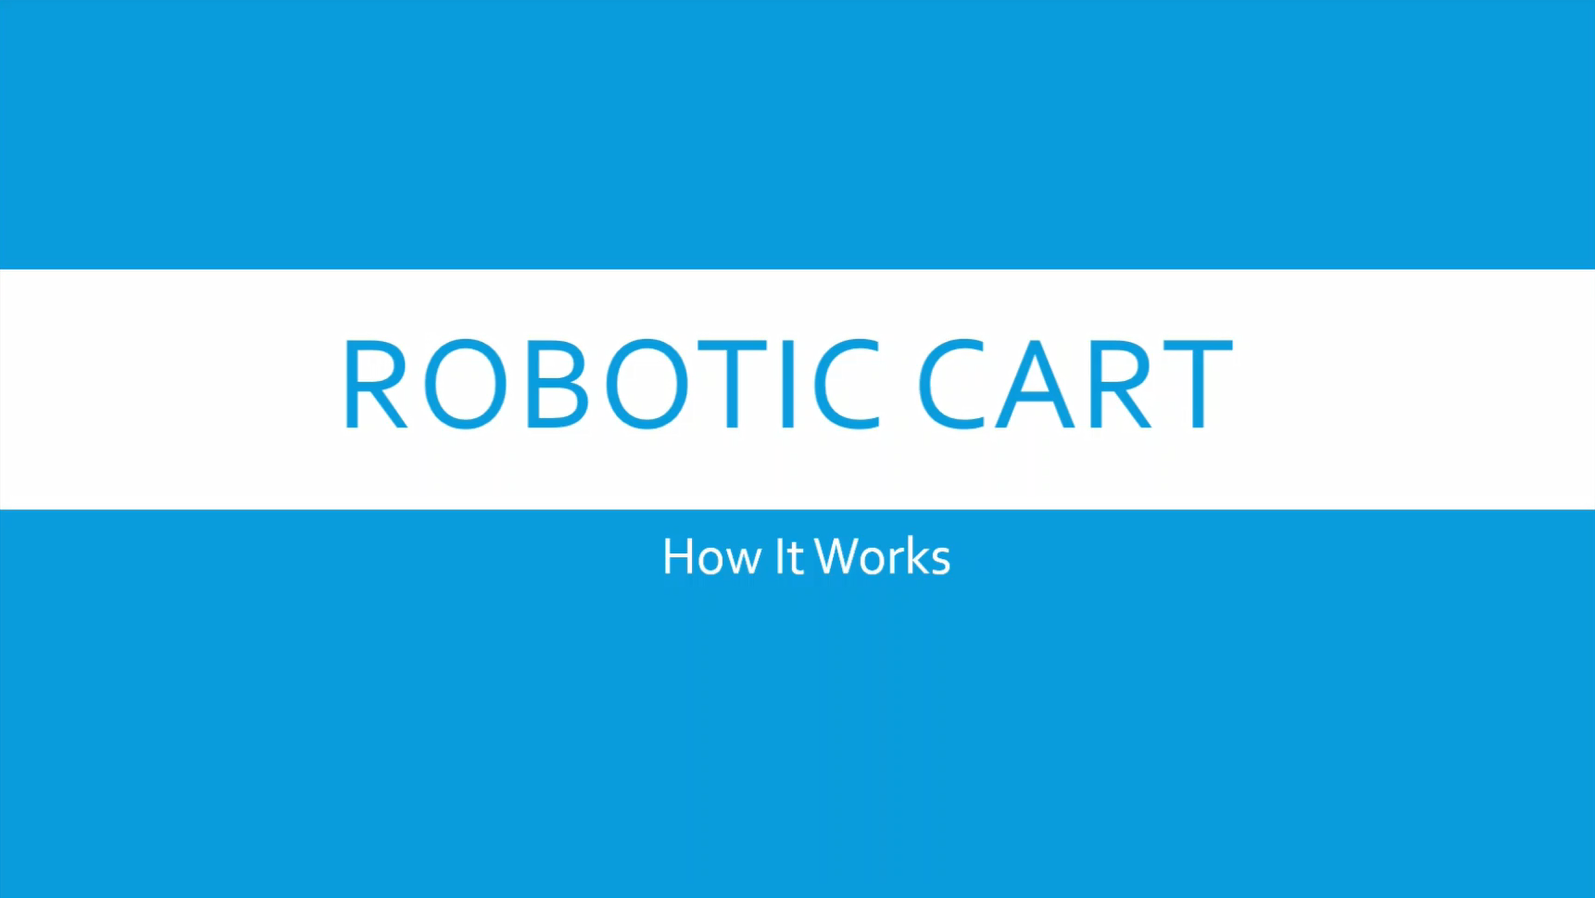
\includegraphics[width=0.8\textwidth]{figs/img/proposalVideoTitle}}
  \end{center}
\end{frame}

\begin{frame}{Introduction}{Problem Statement}
  \begin{block}{Problem Statement}
    \begin{LARGE}
      Design a robotic cart that follows the user without line of sight sensors.
    \end{LARGE}
  \end{block}
  \pause
  \begin{block}{Proposed Solution}
    \begin{LARGE}
      Utilize wireless signal strength to locate and then follow the user.
    \end{LARGE}
  \end{block}
\end{frame}

%----------------------------------

\begin{frame}{Introduction}{}
%\documentclass{beamer}
  % applications of mobile robot navigation and problem description
  \begin{block}{Applications of Mobile Carts}
    \begin{itemize}
      %\item Mail delivery
      %\item Transferring files in offices
      \item Carrying medical supplies in hospitals (Fig.\ref{fig:medCart})
      \item Carrying materials and tools in factories (Fig. \ref{fig:factCart})
      \item Shopping carts for ease of use and people with disabilities
    \end{itemize}
  \end{block}
      \begin{figure}
      \centering
      \begin{minipage}[t]{0.5\textwidth}
        \centering
        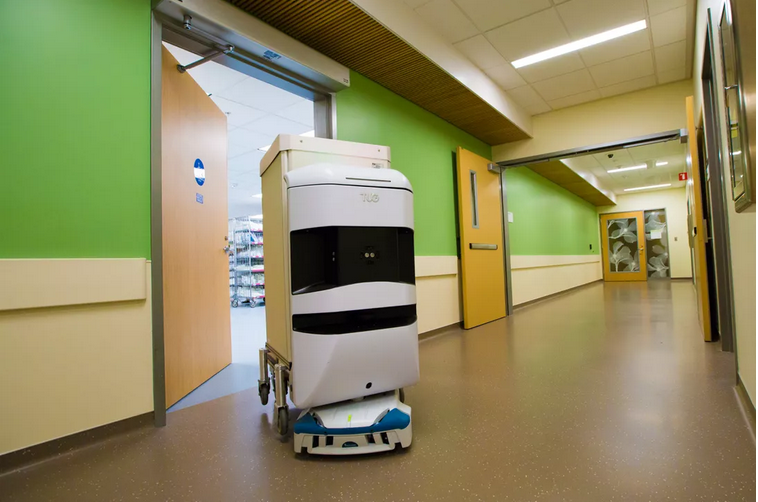
\includegraphics[height=3.0cm]{figs/img/MedicalRoboticCart}
        \caption{Medical Mobile Robotic Cart\textsuperscript{a}}
        \label{fig:medCart}
      \end{minipage}
      \begin{minipage}[t]{0.4\textwidth}
        \centering
        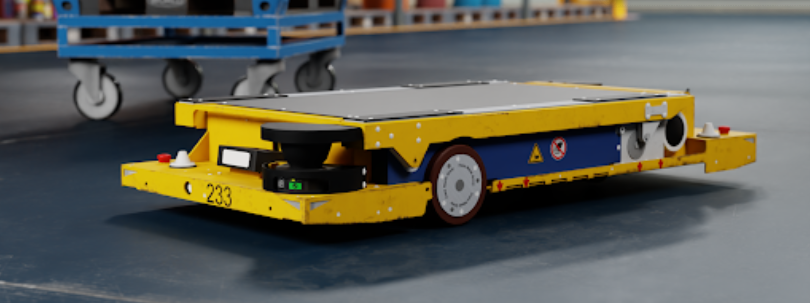
\includegraphics[height=2.0cm]{figs/img/FactoryRoboticCart}
        \caption{Factory Mobile Robotic Cart\textsuperscript{b}}
        \label{fig:factCart}
      \end{minipage}
      \end{figure}
    \begin{tiny}
      \textsuperscript{a}https://www.cnet.com/news/robots-give-a-helping-hand-in-san-franciscos-newest-hospital/\\
      \textsuperscript{b}https://www.greencarcongress.com/2020/05/20200515-nvidia.html
    \end{tiny}
\end{frame}

%----------------------------------

\begin{frame}{Introduction}{Previous Work}
  \begin{block}{Existing Solution}
        Mobile platform interface with ultrasound and radio transmission technology~\cite{Sales2016-CompaRob}
  \end{block}
    \begin{figure}[b]
        \centering
        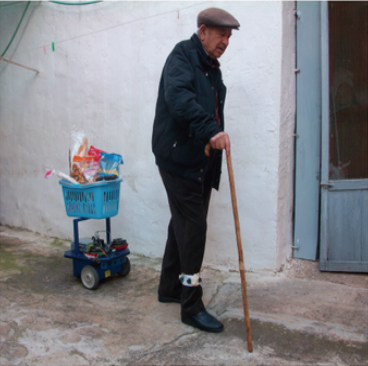
\includegraphics[width=0.4\textwidth]{figs/img/CompaRob}
        \caption{CompaRob}
        %\label{fig:sysBlockDiag}
    \end{figure}
\end{frame}

%----------------------------------

\begin{frame}{Introduction}{Previous Work}
  \begin{block}{Existing Solution}
        Gated Recurrent Unit (GRU) network with LiDAR sensor and camera to map the customer~\cite{islam_lam_fukuda_kobayashi_kuno_2019}
  \end{block}
    \begin{figure}[b]
        \centering
        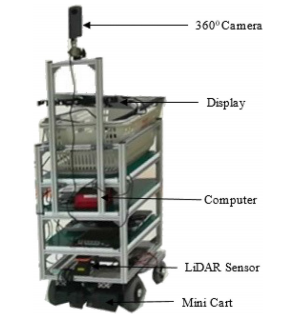
\includegraphics[width=0.38\textwidth]{figs/img/ShoppingSuportRobot}
        \caption{Shopping Support Robot}
        %\label{fig:sysBlockDiag}
    \end{figure}
\end{frame}

%----------------------------------

\begin{frame}{Introduction}{Previous Work}
  \begin{block}{Existing Solution}
    Arduino MEGA 2560, six ultrasonic sensors, two DC motors with Pulse Width Modulation (PWM), an Android Studio IDE device, and Bluetooth~\cite{Rawashdeh2017-Person}
  \end{block}
    \begin{figure}[b]
        \centering
        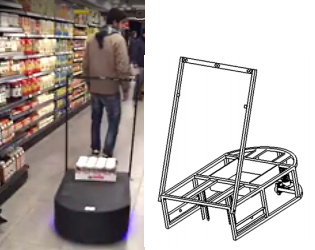
\includegraphics[width=0.45\textwidth]{figs/img/SmartCart}
        \caption{Smart Cart Robot}
        %\label{fig:sysBlockDiag}
    \end{figure}
\end{frame}

%----------------------------------

\begin{frame}{Introduction}{Existing Solutions}
  \begin{block}{Current Problems}
    \begin{itemize}
      \item Require line-of-sight between robot and user
      \item Some require costly dedicated sensors and hardware
    \end{itemize}
  \end{block}
  \pause
  \begin{block}{Benefits of Proposed Solution}
    \begin{itemize}
      \item Line-of-sight is not required since analog RF signals will be used
      \item RF components are cost-effective
    \end{itemize}
  \end{block}
\end{frame}

%----------------------------------

\begin{frame}{Introduction}{System Requirements}
  \begin{block}{Specifications}
    \begin{itemize}
      \item Cart should be able to follow the remote target
      \item Cart should maintain a distance of 1~[\si{\meter}] to 1.5~[\si{\meter}] from the remote target.
      \item Cart should be able to attain a speed of at least 1~[\si{\meter\per\second}]
      \item Cart should not require line-of-sight to follow remote
     \end{itemize}
  \end{block}
\end{frame}

%----------------------------------

\begin{frame}{Introduction}{Challenges}
  \begin{block}{Challenges}
    \begin{itemize}
      \item Accuracy of angle estimation fluctuates and causes some errors in the robots trajectory to the remote
      \item Distance estimation is not consistent and will drastically change if the user stands between the remote and the robot
    \end{itemize}
  \end{block}
\end{frame}

%----------------------------------

\begin{frame}{Introduction}{Nomenclature}
    \begin{itemize}
      \item[]\textbf{RF} - Radio Frequency
      \item[]\textbf{LoS} - Line of Sight
    \end{itemize}
    \bigbreak
    
    \begin{itemize}
      \item[]$K_v$ - proportional gain for linear velocity
      \item[]$K_\omega$ - proportional gain for angular velocity
      \item[]$\theta_r$ - angle of the remote with respect to robot
      \item[]$d_r$ - distance from robot to remote
     \end{itemize}
\end{frame}


%------------------------------------------------------------------------------
%     SECTION BREAK
%------------------------------------------------------------------------------

\section{System Architecture}

\subsection{Block Diagrams}
\begin{frame}{Block Diagrams}
  \begin{block}{}
    Two main components of system
    \begin{itemize}
      \item Mobile Cart
      \item Remote Target
    \end{itemize}
    System Block Diagram shown in Figure \autoref{fig:sysBlockDiag}
  \end{block}
  \begin{figure}[b]
    \centering
    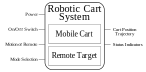
\includegraphics[width=0.75\textwidth]{figs/system_block_diagram_2}
    \caption{Block Diagram of the Robotic Cart System}
    \label{fig:sysBlockDiag}
  \end{figure}
\end{frame}

%----------------------------------

\begin{frame}{Block Diagrams}
  \begin{block}{}
    Remote Target Subsystem Block Diagram shown in Figure \autoref{fig:sysRemoteBlockDiag}
  \end{block}
  \begin{figure}[b]
    \centering
    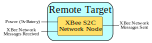
\includegraphics[width=\textwidth]{figs/remote_target_block_diagram}
    \caption{Block Diagram of Remote Target Subsystem}
    \label{fig:sysRemoteBlockDiag}
  \end{figure}
\end{frame}

%----------------------------------

\begin{frame}{Block Diagrams}
  \begin{block}{}
    Mobile Cart Subsystem Block Diagram shown in Figure \autoref{fig:sysMobileBlockDiag}
  \end{block}
  \begin{figure}[b]
    \centering
    \includegraphics[width=0.9\textwidth]{figs/mobile_cart_block_diagram}
    \caption{Block Diagram of Mobile Cart Subsystem}
    \label{fig:sysMobileBlockDiag}
  \end{figure}
\end{frame}

%----------------------------------

\subsection{System Components}
\begin{frame}{System Components}
  \begin{block}{Main Components}
    \begin{itemize}
      \item Budget Bot Chassis - Physical framework of robotic cart (Fig. \ref{fig:budgetBotChassis})
      \item BeagleBone Blue - Embedded computer to control robotic cart (Fig. \ref{fig:beagleboneBlue})
      \item XBee S2C Module - Wireless communication module (Fig. \ref{fig:XBeeModule})
    \end{itemize}
  \end{block}
  \begin{figure}
    \centering
    \begin{minipage}[t]{0.32\textwidth}
      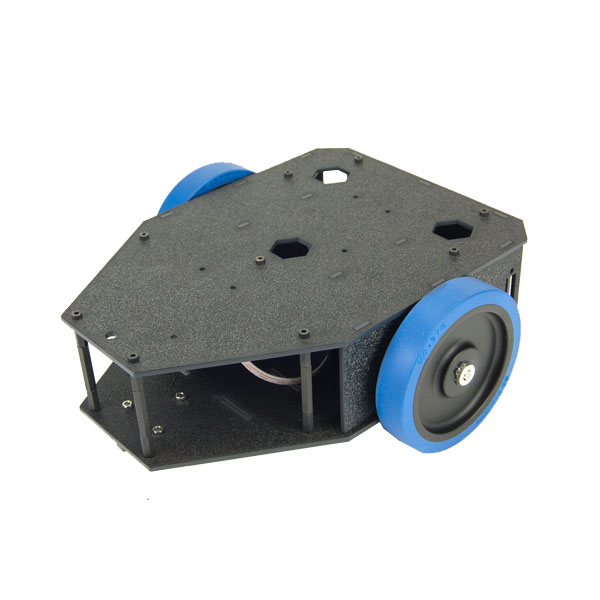
\includegraphics[width=1\textwidth]{figs/img/budgetbot_chassis}
      \caption{Budget Bot Chassis}
      \label{fig:budgetBotChassis}
    \end{minipage}%
    \begin{minipage}[t]{0.32\textwidth}
      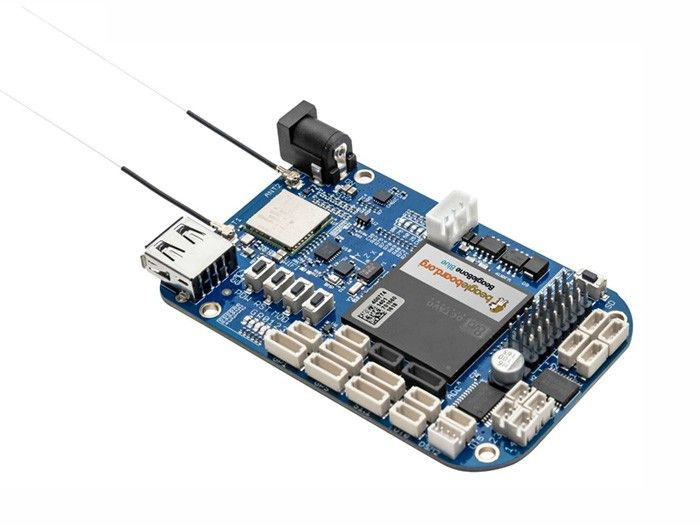
\includegraphics[width=1\textwidth]{figs/img/beaglebone_blue}
      \caption{BeagleBone Blue}
      \label{fig:beagleboneBlue}
    \end{minipage}
    \begin{minipage}[t]{0.32\textwidth}
      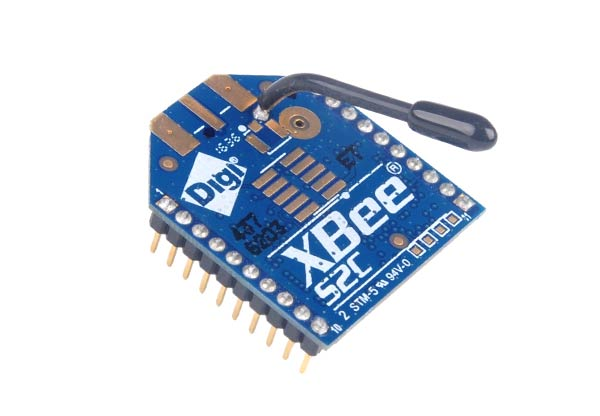
\includegraphics[width=1\textwidth]{figs/img/Xbee-S2C-Module}
      \caption{XBee S2C Module}
      \label{fig:XBeeModule}
    \end{minipage}
  \end{figure}
\end{frame} 

%----------------------------------

\begin{frame}{System Components}
    \begin{block}{Reflector Array}
    Two designs for reflector array:
    \begin{itemize}
      \item Paraboloidal Reflector - Focuses signals coming directly into reflector (Fig. \ref{fig:parabolodialReflector})
      \item Parabolic/Paraboloidal Reflector - Better reception of signals from above (Fig. \ref{fig:parabolicReflector})
    \end{itemize}
    \end{block}
    \begin{figure}
      \centering
      \begin{minipage}[t]{0.5\textwidth}
        \centering
        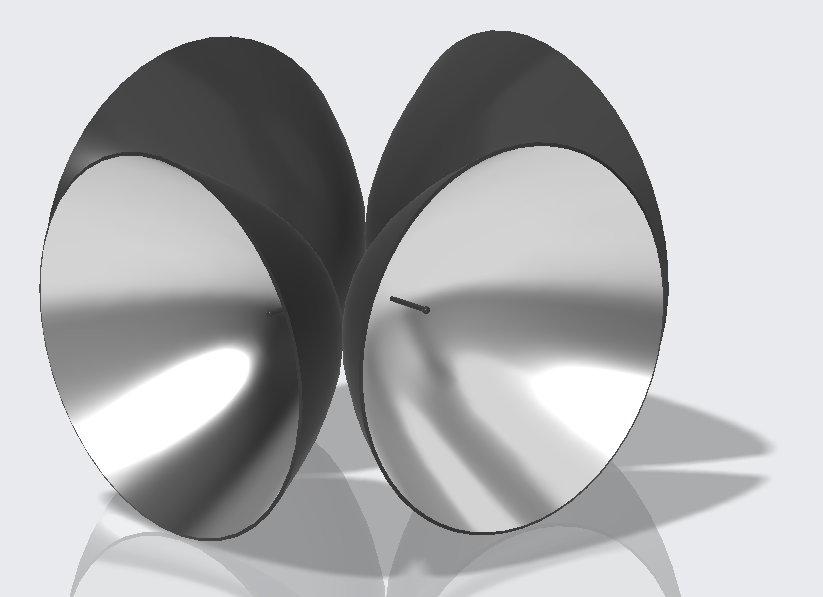
\includegraphics[height=3.5cm]{figs/img/paraboloidalReflector}
        \caption{Paraboloidal Reflector Model}
        \label{fig:parabolodialReflector}
      \end{minipage}
      \begin{minipage}[t]{0.4\textwidth}
        \centering
        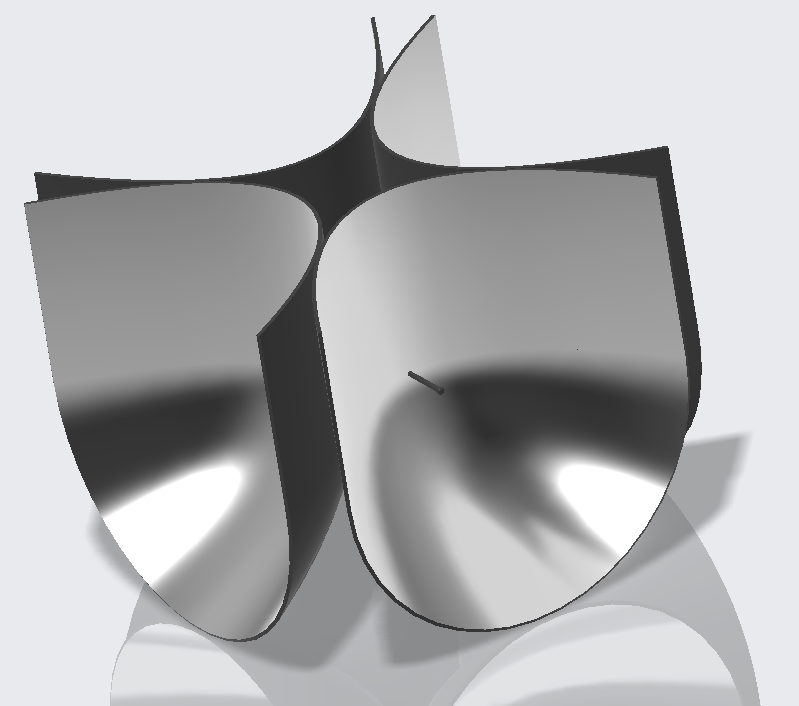
\includegraphics[height=3.5cm]{figs/img/parabolicReflector}
        \caption{Combined Parabolic/Paraboloidal Reflector}
        \label{fig:parabolicReflector}
      \end{minipage}
    \end{figure}
\end{frame}

%----------------------------------

\setlength{\dashlinedash}{2pt}
\setlength{\dashlinegap}{4pt}
\setlength{\arrayrulewidth}{0.3pt}

\begin{frame}{System Components}
  \begin{table}[h!]
      \centering
      \begin{tabular}{c|c}
          \toprule
          \textbf{Quantity} & \textbf{Parts}\\
          \toprule
          2 & Budget Bot Chassis\\
          2 & Battery Packs for Budget Bot\\
          4 & 10 uF Ceramic Capacitor\\
          4 & LM1117 Regulator\\
          2 & 7.4V LiPo Batteries\\
          4 & 5.5 x 8.2 x 0.85 cm Mini Breadboard\\
          3 & XBee USB Adapter\\
          \bottomrule
          %\multicolumn{2}{r|}{\textbf{Total}} & \$ 562.34\\
          %\bottomrule
      \end{tabular}
      \caption{Parts Available in Laboratory}
      \label{tab:Partslablist}
  \end{table}
\end{frame}

%----------------------------------

\begin{frame}{System Components}
  \begin{table}[h!]
    \centering
    \small
    \begin{tabular}{c|c|c|c}
      \toprule
      \textbf{Quantity} & \textbf{Parts} & \textbf{Price} & \textbf{Total}\\
      \toprule
      12 & XBee S2C Module & \$ 23.10 & \$ 277.20\\
      12 & XBee Adapter Board & \$ 4.99 & \$ 59.88\\
      4 & Pololu 37D Metal Gearmotor 4751 & \$ 39.95 & \$ 159.80\\
      2 & Ovonic 7.4V 8,000mAh LiPo Battery & \$ 43.99 & \$ 87.98\\
      2 & Twotrees 4 Lead Nema 17 Stepper Motor & \$ 9.99 & \$ 19.98\\
      2 & DG409DJ+ Multiplexer & \$ 9.07 & \$ 18.14\\
      1 & 4-Pin JST SH Connector - 20 Pack & \$ 7.99 & \$ 7.99\\
      1 & 6-Pin JST SH Connector - 10 Pack & \$ 9.99 & \$ 9.99\\
      1 & Aluminum Foil Tape - 2 in x 5 yd & \$ 6.05 & \$ 6.05\\
      \bottomrule
      \multicolumn{3}{r|}{\textbf{Sub Total}} & \$ 653.88\\
      \bottomrule
    \end{tabular}
    \caption{Purchased parts for the Robotic Cart Project}
    \label{tab:Partslist}
  \end{table}
\end{frame}
 

%------------------------------------------------------------------------------
%     SECTION BREAK
%------------------------------------------------------------------------------

\section{Customized Reflector Array}

\begin{frame}{Customized Reflector Array}
  \begin{columns}
    \column{0.6\textwidth}
      \begin{block}{Problem}
        \begin{itemize}
          \item XBee S2C modules are omnidirectional
          \item Need to know direction of signals
        \end{itemize}
      \end{block}
   \column{0.4\textwidth}
     \begin{figure}
    	\centering
    	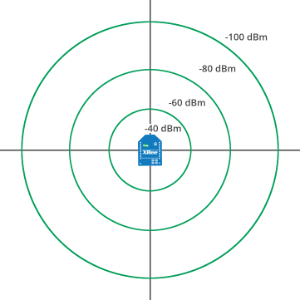
\includegraphics[height=0.5\textheight]{figs/img/XBee_signal.png}
    	\caption{XBee Signal Broadcast Range}
    	\label{fig:XBeeSignal}
  	  \end{figure}
  \end{columns}
\end{frame}

\begin{frame}{customized Reflector Array}
  \begin{columns}
    \column{0.6\textwidth}
      \begin{block}{Problem}
        \begin{itemize}
          \item XBee S2C modules are omnidirectional
          \item Need to know direction of signals
        \end{itemize}
      \end{block}
      \begin{block}{Solution}
        Use a parabolic reflector
        \begin{itemize}
          \item Reduces signal from behind reflector
          \item Maximizes signal entering parallel to axis of parabola
        \end{itemize}
      \end{block}
    \column{0.4\textwidth}
      \begin{figure}
        \centering
        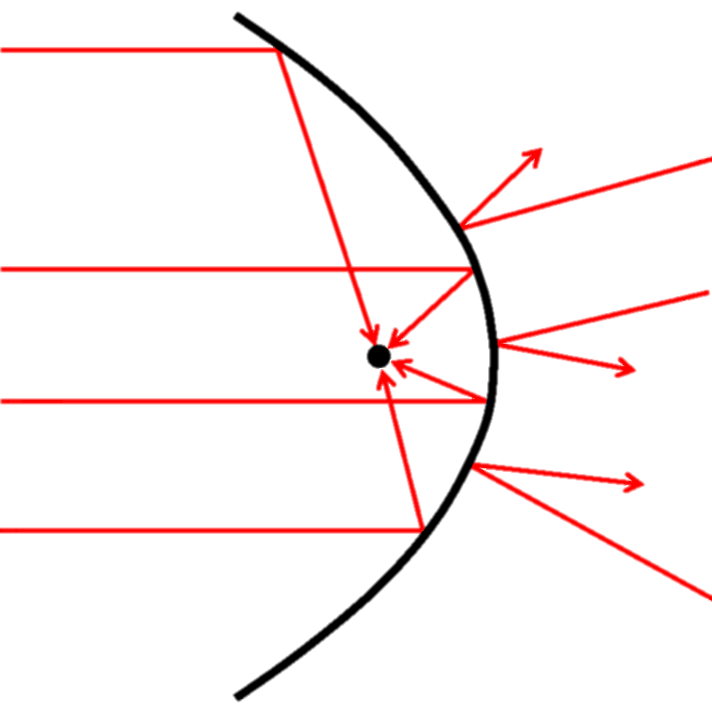
\includegraphics[width=0.9\textwidth]{figs/img/parabolicReflectorDiagram.png}
        \caption{Parabolic Reflector Characteristics}
        \label{fig:parabolicReflectorDiagram}
      \end{figure}
  \end{columns}
\end{frame}

\begin{frame}{Customized Reflector Array}
  \begin{block}{Paraboloidal Reflector Design}
    \begin{itemize}
      \item Maximizes signals entering perfectly horizontally
      \item Works best if remote is held at same level as robot
      \item Shown in Fig. \ref{fig:reflectorDesign1}
    \end{itemize}
  \end{block}
  \begin{figure}
    \centering
    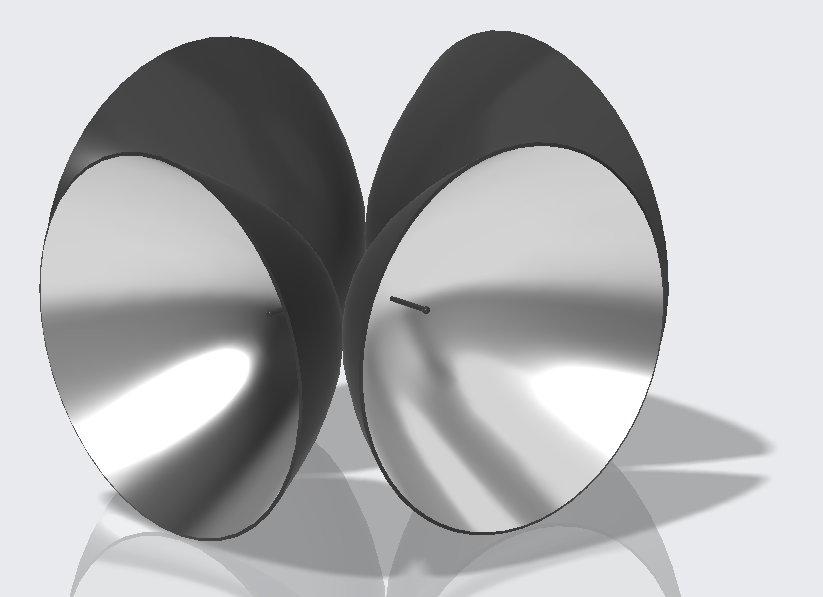
\includegraphics[height=0.5\textheight]{figs/img/paraboloidalReflector.png}
    \caption{Paraboloidal Reflector}
    \label{fig:reflectorDesign1}
  \end{figure}
\end{frame}

\begin{frame}{Customized Reflector Array}
  \begin{block}{Parabolic/Paraboloidal Reflector Design}
    \begin{itemize}
      \item Maximizes signals entering directly in line with reflector
      \item Allows remote to be held higher than the robot
      \item Shown in Fig. \ref{fig:reflectorDesign2}
    \end{itemize}
  \end{block}
  \begin{figure}
    \centering
    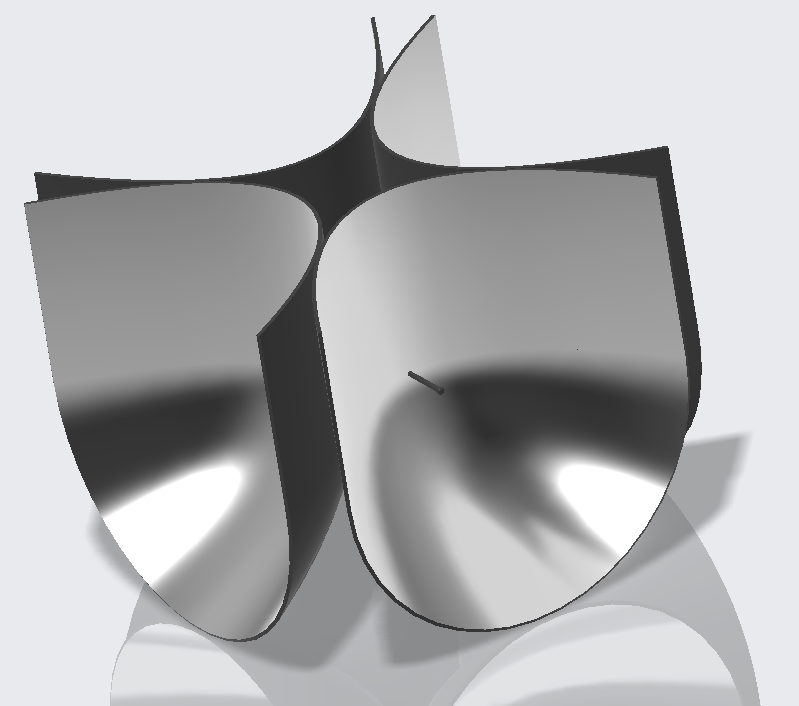
\includegraphics[height=0.5\textheight]{figs/img/parabolicReflector.png}
    \caption{Parabolic/Paraboloidal Reflector}
    \label{fig:reflectorDesign2}
  \end{figure}
\end{frame}

\begin{frame}{Customized Reflector Array}
  \begin{block}{Reflector Construction}
    \begin{itemize}
      \item 3D printed parts (dishes, top and bottom frames)
      \item Lined dishes with foil tape
      \item Fastened parts together with M3 screws and nuts
    \end{itemize}
  \end{block}
  \begin{figure}
    \centering
    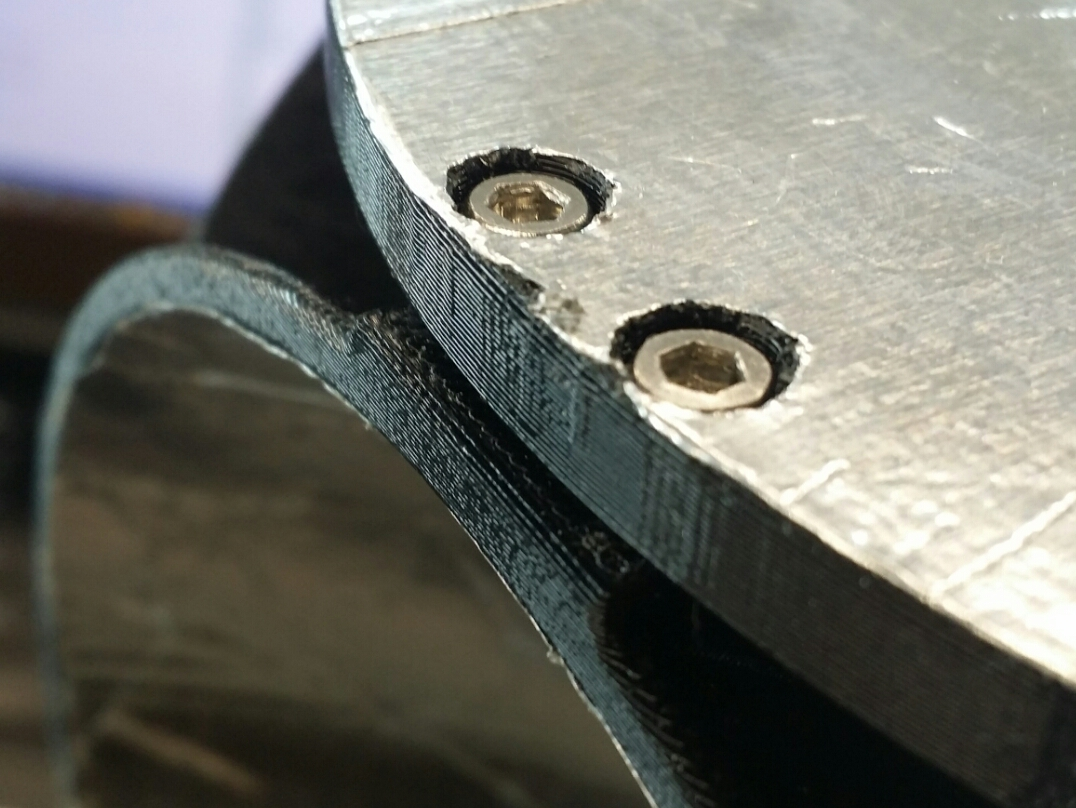
\includegraphics[height=0.5\textheight]{figs/img/reflectorConstruction.jpg}
    \caption{Reflector Construction}
    \label{fig:reflectorConstruction}
  \end{figure}
\end{frame}

%------------------------------------------------------------------------------
%     SECTION BREAK
%------------------------------------------------------------------------------

\section{Algorithms}

\begin{frame}{Algorithms}{System Operation}
  \begin{figure}
    \centering
    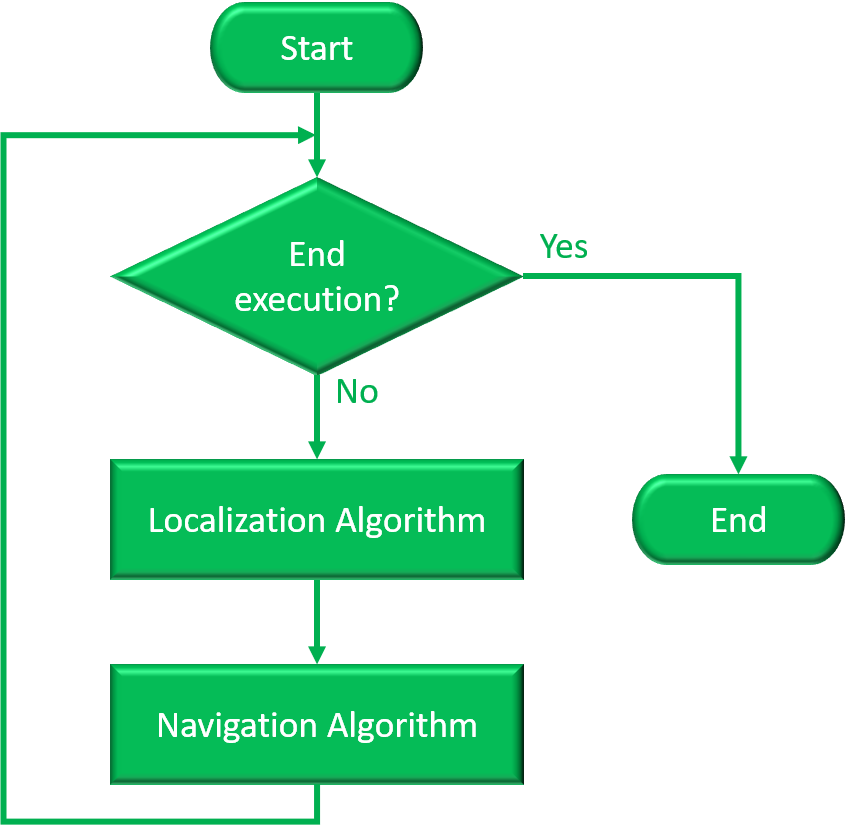
\includegraphics[height=2.5in]{figs/img/systemOperationFlowchart.png}
    \caption{Flowchart of System Operation}
  \end{figure}
\end{frame}

\begin{frame}{Algorithms}{Localization Algorithm}
  \begin{figure}
    \centering
    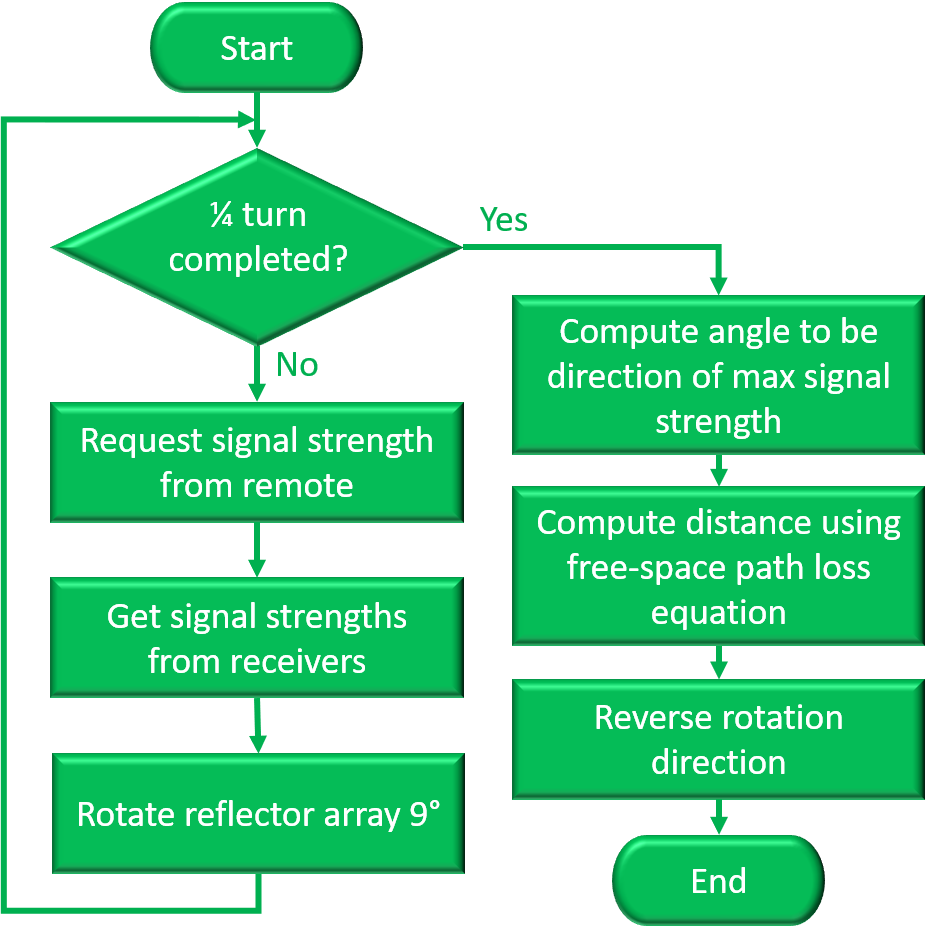
\includegraphics[height=2.5in]{figs/img/localizationAlgoFlowchart.png}
    \caption{Flowchart of Localization Algorithm}
    \label{fig:localizationAlgoFlowchart}
  \end{figure}
\end{frame}

\begin{frame}{Algorithms}{Navigation Algorithm}
  \begin{columns}
    \column{0.6\textwidth}
      \begin{figure}
        \centering
        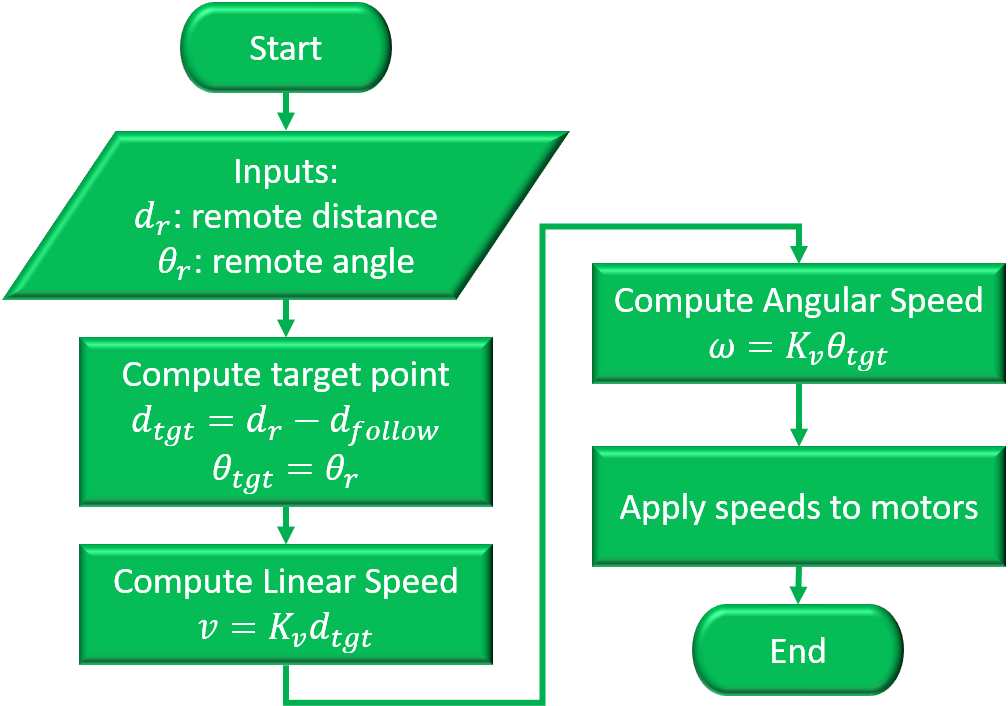
\includegraphics[width=\textwidth]{figs/img/navigationAlgoFlowchart.png}
        \caption{Flowchart of Navigation Algorithm}
        \label{fig:navigationAlgoFlowchart}
      \end{figure}
    \column{0.4\textwidth}
      \begin{figure}
        \centering
        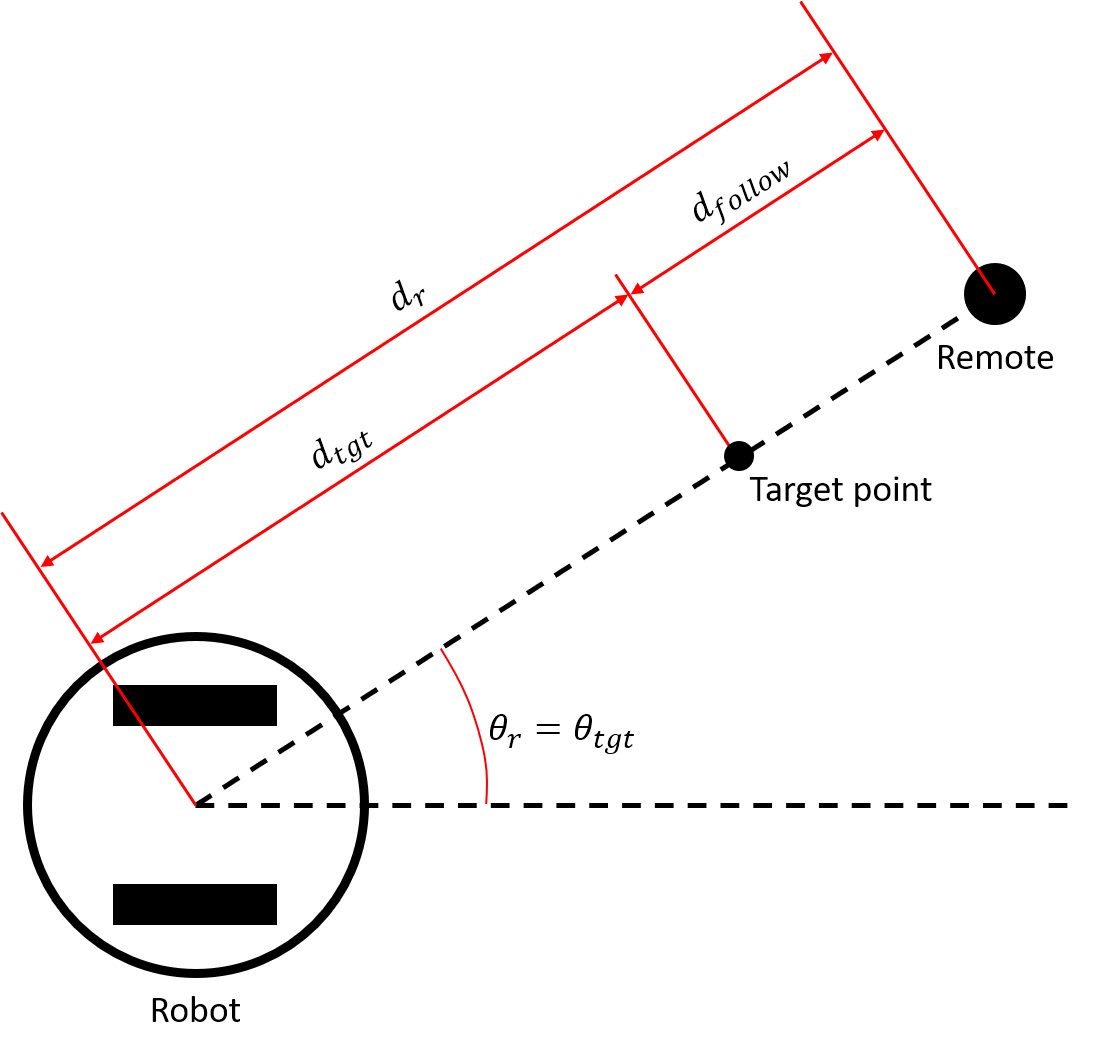
\includegraphics[width=0.9\textwidth]{figs/img/navAlgoDiagram.png}
        \caption{Parameter Diagram}
        \label{fig:navAlgoDiagram}
      \end{figure}
  \end{columns}
\end{frame}

%------------------------------------------------------------------------------
%     SECTION BREAK
%------------------------------------------------------------------------------

\section{Implementation}

\begin{frame}{Implementation}
  
\end{frame}

%------------------------------------------------------------------------------
%     SECTION BREAK
%------------------------------------------------------------------------------

\section{Conclusions and Future Work}

\begin{frame}{Conclusions and Future Work}
  \begin{block}{Future Work}
    \begin{itemize}
      \item Improve the angle estimation calculation
      \item Improve distance calculation by implementing a modified EKF algorithm
      \item Test more variations of parabolic reflectors to see if the XBee signals can be more refined
    \end{itemize}
  \end{block}
\end{frame}

\begin{frame}{Conclusions and Future Work}
  \begin{block}{Conclusions}
    \begin{itemize}
      \item The navigation algorithm we implemented works moderately with only a few errors in the robot's trajectory to the remote
      \item By testing and gathering data we were able to come up with multiple variations of the code that eventually got the robotic cart to move more predictably
      \item In comparison to other robotic carts, our robotic cart was cost effective in it's design
    \end{itemize}
  \end{block}
\end{frame}

%------------------------------------------------------------------------------
%     SECTION BREAK
%------------------------------------------------------------------------------

\section{References}

\begin{frame}{References}
  \bibliographystyle{IEEEtran}
  \bibliography{bib/references.bib}
\end{frame}

%==============================================================================
%==============================================================================
%     END OF SLIDES
%==============================================================================
%==============================================================================

\end{document}

%%% Local Variables:
%%% mode: latex
%%% TeX-master: t
%%% End:
